\documentclass[UTF8]{article}
\usepackage{ctex}
\usepackage{geometry}
\geometry{a4paper, scale=0.8}
\usepackage{graphicx}
\usepackage{subfigure}
\usepackage{float}
\usepackage{enumitem}
\usepackage{amsmath}
\usepackage{amssymb}
\usepackage{amstext}
\usepackage{fontspec}
\newfontfamily\jetbrains{JetBrains Mono}
\usepackage{listings}
\lstset{
    breaklines,                                 % 自动将长的代码行换行排版
    extendedchars=false,                        % 解决代码跨页时,章节标题,页眉等汉字不显示的问题
    backgroundcolor=\color[rgb]{0.96,0.96,0.96},% 背景颜色
    keywordstyle=\color{blue}\bfseries,         % 关键字颜色
    identifierstyle=\color{black},              % 普通标识符颜色
    commentstyle=\color[rgb]{0,0.6,0},          % 注释颜色
    stringstyle=\color[rgb]{0.58,0,0.82},       % 字符串颜色
    showstringspaces=false,                     % 不显示字符串内的空格
    numbers=left,                               % 显示行号
    numberstyle=\tiny\jetbrains,                    % 设置数字字体
    basicstyle=\small\jetbrains,                    % 设置基本字体
    captionpos=t,                               % title在上方(在bottom即为b)
    frame=single,                               % 设置代码框形式
    rulecolor=\color[rgb]{0.8,0.8,0.8},         % 设置代码框颜色
}
\usepackage[colorlinks,linkcolor=blue]{hyperref}

\title{人工智能基础第一次实验报告}
\author{PB19071405\ 王昊元}
\date{2022 年 06 月 28 日}

\begin{document}
    \maketitle

    \section{实验内容}
    \subsection{传统机器学习}
    在不使用任何机器学习库的情况下,手动实现决策树和支持向量机。
    \begin{itemize}
        \item 在决策树部分,你需要通过病人的生理状况、临床观察症状等来推断病人是否癌症复发。
        每个样本由9个离散属性组成,值数在2-12不等,标签包括癌症复发或不复发,取值为\{0,1\},是一个二分类任务。
        \item 在支持向量机部分,你需要根据病人的生理指标预测在给定的时间中病人是否会死亡。
        我们将其抽象成一个二分类问题:输入生理指标与给定的时间,模型将其分类为死亡或未死亡。
        每个样本具有7个数值型属性,包括年龄,射血分数,血小板数以及给定的时间等等。
        所有数据类型均为浮点数,且数值在-10到10之间。
        标签即为患者在给定的时间中是否死亡,1表示已死亡,-1表示未死亡。
        使用\{-1,1\}作为标签集便于SVM的处理。
    \end{itemize}
    \subsection{深度学习}
    \begin{itemize}
        \item 实现一个5层的感知机模型(输入层为10,隐层神经元设置为10,8,8,输出层为4,即输入的特征个数为10,输出的类别个数为4,激活函数设置为tanh);
        实现mlp前向传播算法,及反向传播和梯度下降算法。
        要求通过矩阵运算实现模型,实现各参数的梯度计算,给出各参数矩阵的梯度,
        并与pytorch自动计算的梯度进行对比,实现梯度下降算法优化参数矩阵,给出loss的训练曲线。
        \item 在给定框架下,根据自己的学号及要求,实现对应的卷积神经网络模型。
    \end{itemize}
    \section{实验环境}
    \begin{itemize}
        \item Python 3.9.12(所使用包版本可以参考{\jetbrains requirements.txt})
        \item venv虚拟环境管理工具
        \item macOS Version 11.2.3
        \item 1.8 GHz Dual-Core Intel Core i5
    \end{itemize}
    \section{实验实现}
    \subsection{决策树}
    采用自顶向下递归构建的方式,实现了一个二叉决策树,根据不同属性对于所对应阈值构建二叉决策树。
    思路是对于每个属性的每一种取值,尝试作为阈值(分界点),计算信息增益,
    记录信息增益最大的一种属性及相应阈值,然后分别对在这种区分方式下的两部分数据递归构造决策树。
    \begin{lstlisting}[language=python]
for feature_idx in range(num_features):
    # feature_vals.shape (num_samples, 1)
    feature_vals = np.expand_dims(features[:, feature_idx], axis=1)
    # unique_vals is the all values of this feature
    unique_vals = np.unique(feature_vals)
    for value in unique_vals:
        logging.debug(f"feature_idx: {feature_idx}")
        logging.debug(f"value: {value}")
        logging.debug(f"features_labels[:, feature_idx]: {features_labels[:, feature_idx]}")
        fl_less_than_value = features_labels[
            features_labels[:, feature_idx] < value
        ]
        fl_not_less_than_value = features_labels[
            features_labels[:, feature_idx] >= value
        ]
        logging.debug(f"{fl_less_than_value.size > 0 and fl_not_less_than_value.size > 0}")
        if fl_less_than_value.size > 0 and fl_not_less_than_value.size > 0:
            # label_less_than_value = fl_less_than_value[:, num_features:]
            # label_not_less_than_value = fl_not_less_than_value[:, num_features:]
            label_less_than_value = np.expand_dims(fl_less_than_value[:, -1], axis=1)
            label_not_less_than_value = np.expand_dims(fl_not_less_than_value[:, -1], axis=1)
            info_gain = DecisionTree.calc_info_gain(labels, label_less_than_value, label_not_less_than_value)
            logging.debug(f"info_gain: {info_gain}")
            if info_gain > info_gain_max:
                info_gain_max = info_gain
                best_feature_idx = feature_idx
                best_threshold = value
                best_division = (fl_less_than_value, fl_not_less_than_value)
    \end{lstlisting}
    \subsection{支持向量机}
    利用助教实现的核函数类,进行核矩阵的构建。
    \begin{lstlisting}[language=python]
num_samples = train_data.shape[0]
# init kernel matrix
kernel_matrix = np.zeros((num_samples, num_samples))
for i in range(num_samples):
    for j in range(num_samples):
        kernel_matrix[i, j] = self.KERNEL(train_data[i], train_data[j])
    \end{lstlisting}

    利用{\jetbrains cvxopt.solvers.qp}进行SVM凸优化问题的求解,对应问题形式如下:
    \begin{figure}[H]
        \centering
        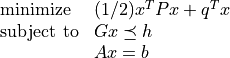
\includegraphics[]{./figs/cvxopt_qp.png}
        \caption{官方的问题形式}
    \end{figure}
    老师提供的slides上的软间隔SVM凸优化问题的对偶问题如下:
    \begin{figure}[H]
        \centering
        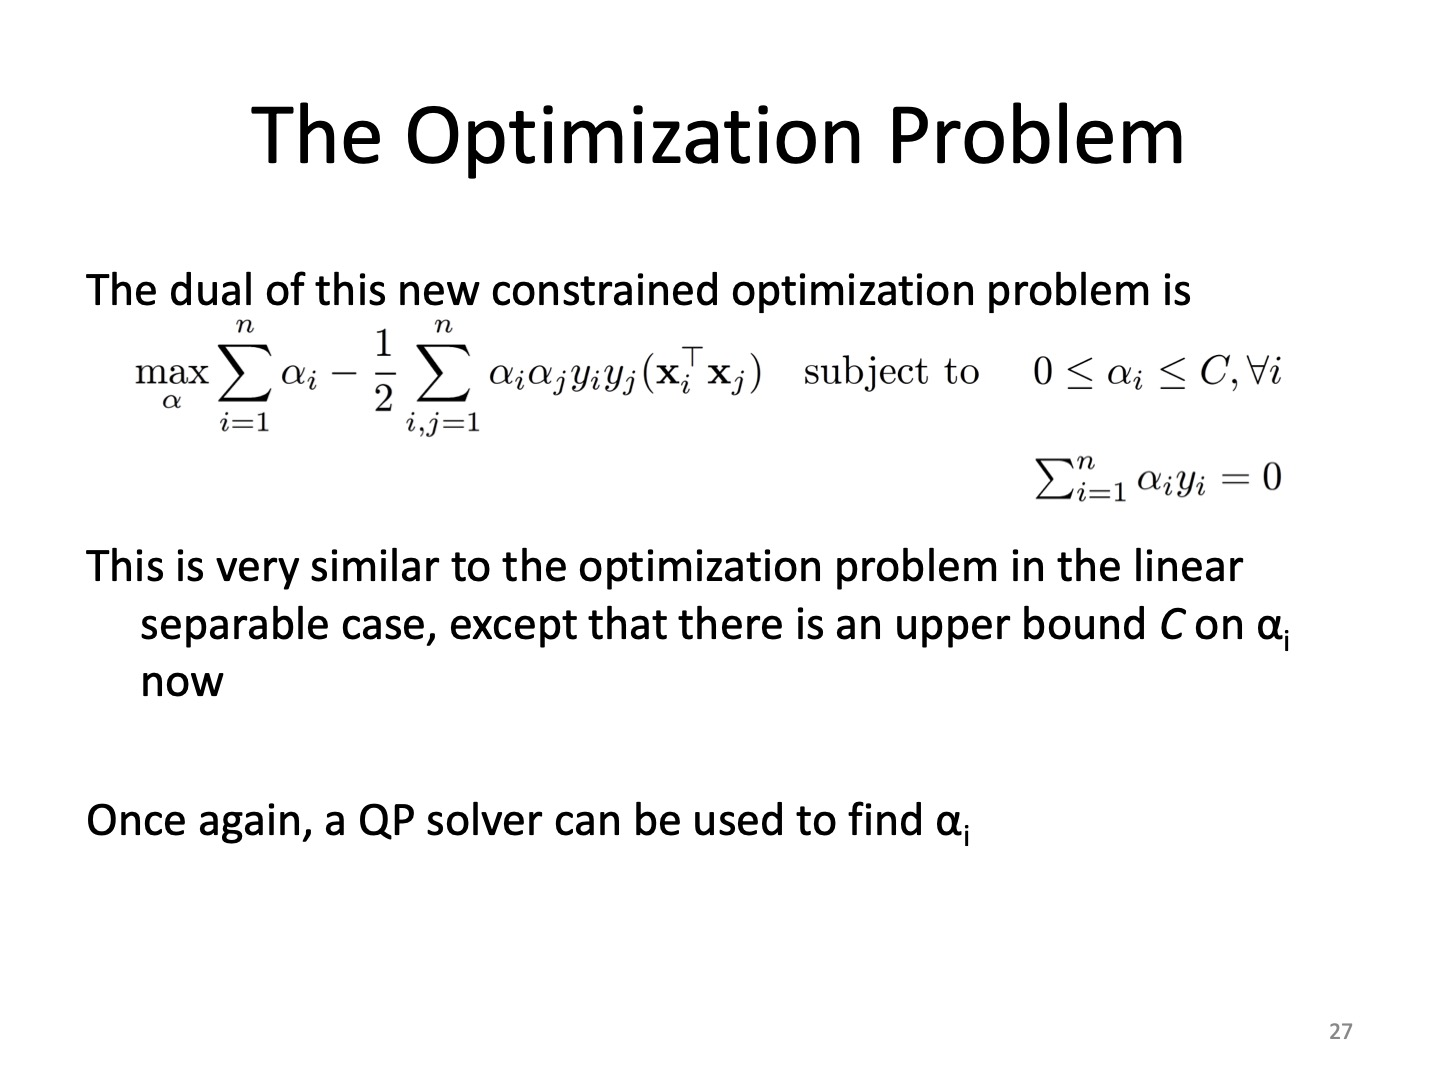
\includegraphics[width=0.7\textwidth]{./figs/soft_svm_from_slides.jpg}
        \caption{来自于课程slides上的凸优化问题的对偶问题}
    \end{figure}
    对比可以实现软间隔SVM的求解,如下:
    \begin{lstlisting}[language=python]
# 凸优化问题求解
P = cvxopt.matrix(np.outer(train_label, train_label) * kernel_matrix, tc='d')
q = cvxopt.matrix(np.ones(num_samples) * -1)
A = cvxopt.matrix(train_label, (1, num_samples), tc='d')
b = cvxopt.matrix(0, tc='d')
G = cvxopt.matrix(np.concatenate((np.identity(num_samples) * -1, np.identity(num_samples)), axis=0))
h = cvxopt.matrix(np.concatenate((np.zeros(num_samples), np.ones(num_samples) * self.C), axis=0))
cvxopt.solvers.options['show_progress'] = False
minimization = cvxopt.solvers.qp(P, q, G, h, A, b)
x = np.ravel(minimization['x'])
sv_idx = x > self.epsilon
# 根据问题结果求解支持向量及其他参数
self.SV = train_data[sv_idx]
self.SV_label = train_label[sv_idx]
self.SV_alpha = x[sv_idx]
self.b = self.SV_label[0]
tmp_matrix = np.zeros((self.SV_alpha.shape[0], self.SV_alpha.shape[0]), dtype=np.float64)
for i, sv in enumerate(self.SV):
    tmp_matrix[i][i] = self.KERNEL(sv, self.SV[0])
self.b -= np.matmul(
    np.matmul(
        self.SV_alpha,
        tmp_matrix,
    ),
    self.SV_label
)
    \end{lstlisting}
    \subsection{手写实现MLP}
    分别定义两个新的类(在mlp类中实现,事实上在哪里定义都可以),
    线性层({\jetbrains LinearLayer})和激活层({\jetbrains Tanh}),
    MLP中的各个层均为这两个类的对象。

    前向传播即对每一层进行一个向前运算({\jetbrains forward})。
    反向传播需要根据每一层的损失(在MLP初始化时定义了交叉熵损失函数)
    和梯度(在计算loss时一起计算即可)
    更新前一层的权重(weights)和偏重(bias,不太清楚这个中文该怎么翻译),
    有点类似于牛顿迭代法的计算。
    需要注意的是所有层同步更新,即由于后一层反向传播造成的影响不会影响该层对后一层的影响。
    \begin{lstlisting}[language=python]
def backward(self, inputs, labels, lr):  # 自行确定参数表
# 反向传播
weights_layers = []
grad_weights_layers = []
biases_layers = []
grad_biases_layers = []
preds = self.forward(inputs)
loss, grad = self.loss(preds, labels)  # softmax_cross_entropy
# reverse layers for back propagation
for layer in reversed(self.layers):
    grad, weights, grad_weights, biases, grad_biases = layer.backward(grad)
    if weights is not None:  # linear layer
        # for updating weights and bias
        # update after the traverse(IMPORTANT POINT)
        weights_layers.append(weights)
        grad_weights_layers.append(grad_weights)
        biases_layers.append(biases)
        grad_biases_layers.append(grad_biases)
for weight, grad_weight, biases, grad_bias in zip(weights_layers, grad_weights_layers, biases_layers, grad_biases_layers):
    weight -= grad_weight * lr
    biases -= grad_bias * lr
return loss
    \end{lstlisting}
    \subsection{卷积神经网络}
    学号为PB19071405,对应第6个模型。
    因为在线性层之前和之后需要对数据进行{\jetbrains view}的操作
    (变成一维数据,线性层的要求),所以将线性层之前的和之后的分开,
    分别使用{\jetbrains nn.Sequential}进行构造。
    \begin{lstlisting}[language=python]
def __init__(self):
    super(MyNet, self).__init__()
    ########################################################################
    # 这里需要写MyNet的卷积层、池化层和全连接层
    """
    学号 PB19071405 对应第6个模型
    layer1: 2d卷积 10,5
    layer2: 平均池化
    layer3: 2d卷积 20,3
    layer4: 平均池化
    layer5: 2d卷积 32,3
    layer6: 线性 120
    layer7: 线性 72
    layer8: 线性 10
    激活函数: tanh
    """
    self.conv = nn.Sequential(
        nn.Conv2d(3, 10, 5),  # layer1
        nn.Tanh(),
        nn.AvgPool2d(2),  # layer2
        nn.Conv2d(10, 20, 3),  # layer3
        nn.Tanh(),
        nn.AvgPool2d(2),  # layer4
        # nn.Conv1d(20, 32, 3),  # layer5
        nn.Conv2d(20, 32, 3),  # layer5
        nn.Tanh(),
    )
    self.linear = nn.Sequential(
        nn.Linear(32 * (((32-4)//2-2)//2-2) * (((32-4)//2-2)//2-2), 120),  # layer6
        nn.Tanh(),
        nn.Linear(120, 72),  # layer7
        nn.Tanh(),
        nn.Linear(72, 10)  # layer8
    ) 
    \end{lstlisting}
    优化器选择{\jetbrains Adam},效果较好。
    \section{实验结果}
    \subsection{决策树}
    \begin{figure}[H]
        \centering
        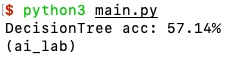
\includegraphics[width=0.7\textwidth]{./figs/decisiontree_result.jpg}
        \caption{决策树的预测结果}
    \end{figure}
    \subsection{支持向量机}
    \begin{figure}[H]
        \centering
        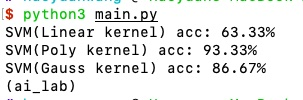
\includegraphics[width=0.7\textwidth]{./figs/svm_result.jpg}
        \caption{软间隔支持向量机的结果}
    \end{figure}
    \subsection{手写实现MLP}
    \begin{figure}[H]
        \centering
        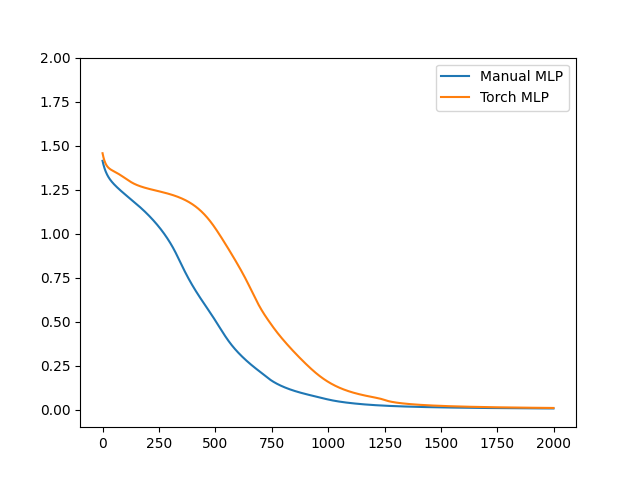
\includegraphics[width=0.7\textwidth]{./figs/mlp.png}
        \caption{手写MLP与利用torch实现的MLP\ loss下降对比}
    \end{figure}
    \subsection{卷积神经网络}
    各层的{\jetbrains weights}和{\jetbrains bias}如下:
    \begin{lstlisting}
Layer 0 weights:
[[ 0.66153737  0.35153786 -0.76296891 -1.06080932  0.02754009 -1.311351
    0.27727742  0.24274614  0.62911964 -0.19553607]
    [ 1.2761464  -0.56817241 -0.20037852 -0.08209294 -0.16873416  0.38701402
    -0.06690592 -0.4307429  -0.20871913  0.26536477]
    [-0.00506159  1.5454856   1.1057474  -0.11272855  0.46875699 -0.14693438
    -0.52884692 -0.63582808  0.46809326  0.28665377]
    [-0.42366498  0.46692603 -1.24809422 -0.87238186 -0.32547721 -0.53787145
    -1.14994503  0.18859783  1.19797802  0.00245439]
    [-0.59203317 -0.53269072 -0.60961857  1.21830635 -0.23350741 -0.66352482
    -0.44097879  1.0578394   0.41246854  0.90154488]
    [ 0.18351266 -1.1047775  -0.83352112  0.15824358 -0.44587536 -0.29767337
    0.10789605  0.50517464 -0.85698783  0.58265063]
    [-0.17209951  0.19659881 -0.22432465  0.22115523  0.48875109  0.33575089
    0.4411111   0.60833641  1.98301533 -0.77973089]
    [-0.68983775  0.54005114  0.0799219   0.14015108  0.31799287 -1.0621606
    -0.23819188  0.40954017 -0.08553607  0.26920776]
    [ 0.55437697  0.00652849  0.2817465   0.72248854  0.1483315  -0.3090718
    -0.25524052  0.43316547  0.4903586   0.57741342]
    [ 0.05777651  0.84355264  0.2501889  -0.60960419  0.42776906 -0.35444244
    -0.67029557 -0.3888594   0.06500947  0.42229289]]
Layer 0 bias:
[[ 0.97254004 -0.38695248 -0.10670324 -0.10717668  0.08536271  0.14247767
    1.03820674  0.02992254 -0.19517793  0.16155655]]
Layer 1 weights:
[[-0.58907317  0.80010546  0.29865274 -0.23742787 -0.83823214  0.08003264
    0.63460204 -0.67513725]
    [-0.62767104  0.6204846  -0.47861443 -0.36217106  0.07735868  0.33598078
    0.12802575 -1.53157913]
    [ 0.62187996 -0.78633351  1.10519681 -0.39538585  0.53626597 -0.73836426
    0.81457037  1.14947028]
    [-1.07374545  1.17081868  0.10663363 -0.50936968 -0.78609351  0.28498507
    0.08908771 -0.3989276 ]
    [-0.56458789  0.8732387   0.08832953 -0.57350263  0.05824795 -0.3235586
    0.40925331 -0.14746161]
    [-0.12810644 -0.15030787  1.5363216  -0.23375404  0.07553462  0.93839064
    0.39869947 -0.72797169]
    [ 0.5770149  -0.47782762  0.0958736  -1.28231578  0.67787467  0.91370412
    0.21237269 -0.22102913]
    [-0.33613301  0.18206412 -0.13046183 -0.96750289 -0.26655324 -0.41139916
    -0.57479614 -1.02192162]
    [ 0.40145319 -1.01766553  0.24708831 -0.15677295  1.048925   -1.34496136
    -0.59393874  1.05804107]
    [ 1.26046835 -0.91589931 -0.48691857 -0.10381662  0.44291681 -0.24789631
    -0.12410921  0.06023536]]
Layer 1 bias:
[[-0.0866818  -0.57298362 -0.70737902 -0.47876405 -0.48608274  0.40735806
    0.08922639  0.36364483]]
Layer 2 weights:
[[-0.64953238  0.68599736 -0.56603047  1.30026573 -0.79658004 -0.33501968
    0.39018498  1.08279442]
    [ 0.64028347 -0.70304136  1.28483086 -0.78933949  1.49787715  0.57492763
    0.21205634 -1.40990914]
    [ 0.03823081  0.73315945  0.14123832  1.08738809 -0.16676636 -0.25955589
    -0.79980309  1.12320505]
    [-0.31753621 -0.36558595 -0.70969743 -0.48033145  0.10335037  0.4825129
    0.25124014 -0.89417182]
    [-0.04044653  0.42723784 -0.51958444  1.07904611 -0.88900061 -0.31132925
    0.34611669  1.04187451]
    [ 0.90016592 -0.56552934  0.975255   -0.60891012 -0.82612455  0.83122367
    -0.20935755  0.1448066 ]
    [-0.59014356 -0.06613788 -0.43431596 -0.17363388  0.72487377  0.25114639
    0.11595427 -0.85505849]
    [-1.5114485   0.32780216 -2.26149293  0.49194706 -0.55014248 -0.62060044
    0.46481733 -0.62639453]]
Layer 2 bias:
[[-0.38175333 -0.45325236 -0.72249973 -0.5581397  -0.58469568  0.20005996
    0.36748717 -0.23568329]]
Layer 3 weights:
[[-1.09676966  1.30388072  0.99039456 -1.20087691]
    [ 1.49672311 -0.34848539 -0.57497837 -0.59456505]
    [-1.96958373  1.99317227  1.40473808 -1.88847069]
    [ 2.45333441  0.04972583 -0.71055594 -1.05469534]
    [-0.53286207 -1.75740717  2.10674738 -0.11613908]
    [-0.79766394  0.5451474   0.62204302  0.1954691 ]
    [-0.23126268 -0.08009554 -0.25633602  1.1444717 ]
    [ 1.50117185  1.54486541 -1.74892331 -1.32752023]]
Layer 3 bias:
[[-0.14731396  0.11914849 -0.61426014  0.64242562]]
    \end{lstlisting}
    \begin{figure}[H]
        \centering
        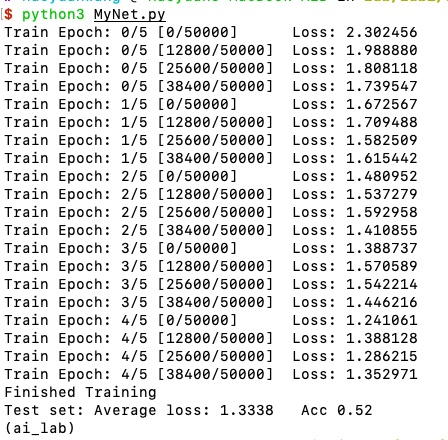
\includegraphics[width=0.7\textwidth]{./figs/mynet_result.jpg}
        \caption{卷积神经网络的预测结果}
    \end{figure}
    \section{实验总结}
    这次实验因为跟别的一些实验同期,导致完成的有些仓促,很多地方完成的不是很好,
    例如在手写MLP部分可以先实现一个表示层的类,再将线性层和激活层作为其子类进行实现,
    又比如决策树并非根据每个属性具体离散值进行决策而是根据属性阈值进行决策,
    有很多想法但没有时间优化或实现。虽然没有做到完美,但我仍收获了很多,了解机器学习和神经网络很多底层的知识。
\end{document}